\documentclass[aspectratio=169,10pt]{beamer}

\usetheme{Madrid}
\usecolortheme{seahorse}

\usepackage[utf8]{inputenc}
\usepackage{amsmath}
\usepackage{amssymb}
\usepackage{amsthm}
\usepackage{mathtools}
\usepackage{xcolor}
\usepackage{listings}
\usepackage{xparse}
\usepackage{tikz}
\usepackage{pgfplots}

\usetikzlibrary{shapes,arrows,positioning}
\pgfplotsset{compat=1.17}

% Beamer customization
\setbeamertemplate{footline}[frame number]
\setbeamertemplate{navigation symbols}{}
\setbeamersize{text margin left=1cm, text margin right=1cm}

\graphicspath{{figures/}}

% Define colors
\definecolor{MyBlue}{RGB}{46,134,171}
\definecolor{MyGreen}{RGB}{6,168,125}
\definecolor{MyOrange}{RGB}{241,143,1}

% Python code style
\lstdefinestyle{mypython}{
    language=Python,
    basicstyle=\ttfamily\scriptsize,
    commentstyle=\color{green!50!black}\itshape,
    keywordstyle=\color{blue}\bfseries,
    stringstyle=\color{red},
    breaklines=true,
    numbers=left,
    numberstyle=\tiny\color{gray},
    frame=single,
    rulecolor=\color{gray},
    showstringspaces=false,
    backgroundcolor=\color{gray!5}
}

% Theorem styles
\newtheorem{proposition}{Proposition}
\newtheorem{definition}{Definition}

% Title page
\title{Chapter 7a: Variational Methods and Optimization}
\subtitle{Existence and Uniqueness of Solutions via Fixed Point Theory}
\author{Based on Pathak's \textit{An Introduction to Nonlinear Analysis and Fixed Point Theory}}
\date{\today}

\begin{document}

% ==============================================================================
% TITLE SLIDE
% ==============================================================================
\begin{frame}
  \titlepage
  \vspace{-0.5cm}
  {\color{MyBlue}\textbf{Topics:}} Variational Principles, Optimization, Ekeland's Theorem, Variational Inequalities
\end{frame}

% ==============================================================================
% OUTLINE
% ==============================================================================
\begin{frame}{Outline and Learning Objectives}
  \tableofcontents

  \vspace{1cm}
  \textbf{Key Learning Objectives:}
  \begin{itemize}
    \item Understand the connection between variational methods and fixed point theory
    \item Master Ekeland's variational principle and its applications
    \item Apply optimization techniques in Banach spaces
    \item Use variational inequalities to establish existence and uniqueness of solutions
  \end{itemize}
\end{frame}

% ==============================================================================
% SECTION 1: VARIATIONAL PRINCIPLES
% ==============================================================================
\section{Variational Principles}

\begin{frame}{Section 7.1: Variational Principles}
  \begin{definition}[Equilibrium Problem (EP)]
    Find $\bar{x} \in K$ such that
    \[
    F(\bar{x}, y) > 0 \quad \text{for all } y \in K.
    \]
  \end{definition}

  \textbf{Significance:} The Equilibrium Problem is a fundamental framework that encompasses many important problems in mathematics and applications.

  \vspace{0.5cm}

  \textbf{Special cases as variational formulations:}
  \begin{itemize}
    \item Minimization problems
    \item Saddle point problems
    \item Nash equilibrium problems
    \item Fixed point problems
  \end{itemize}
\end{frame}

% ==============================================================================
\begin{frame}[allowframebreaks]{Minimization Problem (MP)}
  \begin{definition}[Minimization Problem]
    Find $\bar{x} \in K$ such that
    \[
    \varphi(\bar{x}) \leq \varphi(y) \quad \text{for all } y \in K,
    \]
    where $\varphi: K \to \mathbb{R}$ is a function.
  \end{definition}

  \vspace{0.5cm}

  \textbf{Equivalence to EP:} If we define $F(x, y) = \varphi(y) - \varphi(x)$ for all $x, y \in K$, then the problem (MP) is equivalent to the problem (EP).

  \vspace{0.5cm}

  \begin{center}
    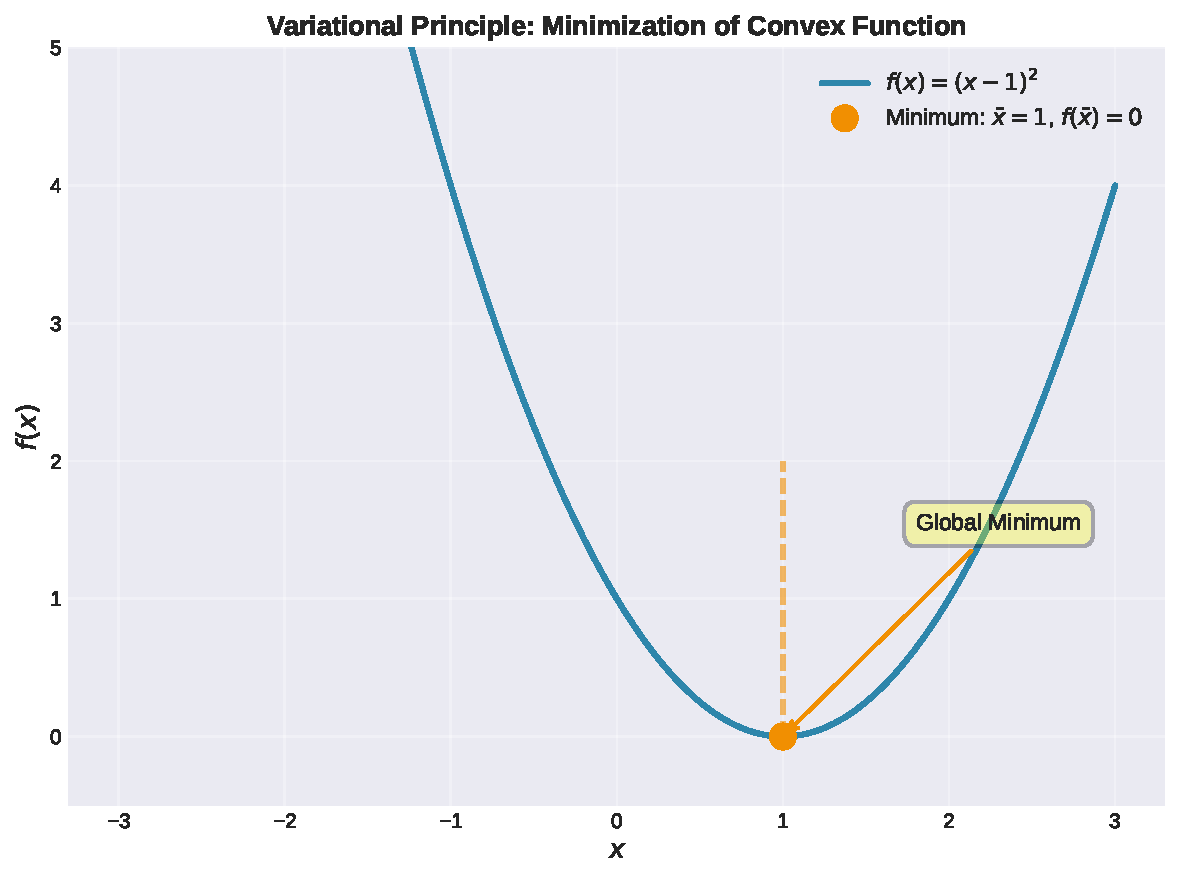
\includegraphics[width=0.65\textwidth]{fig_variational_principle.pdf}
  \end{center}

  \framebreak

  \textbf{Example:} Consider the quadratic optimization problem in $\mathbb{R}^n$:
  \[
  \min_{x \in K} \|Ax - b\|^2
  \]
  where $A \in \mathbb{R}^{m \times n}$ and $b \in \mathbb{R}^m$.

  \vspace{0.3cm}

  The equivalent EP formulation is:
  \[
  F(x, y) = (A(y-x))^T (Ax - b) > 0 \quad \text{for all } y \in K.
  \]
\end{frame}

% ==============================================================================
\begin{frame}[allowframebreaks]{Saddle Point Problem (SPP)}
  \begin{definition}[Saddle Point Problem]
    Find $(\bar{x}_1, \bar{x}_2) \in K_1 \times K_2$ such that
    \[
    L(\bar{x}_1, y_2) \leq L(\bar{x}_1, \bar{x}_2) \leq L(y_1, \bar{x}_2) \quad \text{for all } (y_1, y_2) \in K_1 \times K_2,
    \]
    where $L: K_1 \times K_2 \to \mathbb{R}$ is a real-valued bifunction.
  \end{definition}

  \vspace{0.5cm}

  \textbf{Equivalence to EP:} Define $K = K_1 \times K_2$ and the bifunction:
  \[
  F((x_1, x_2), (y_1, y_2)) = L(y_1, x_2) - L(x_1, y_2).
  \]
  Then the saddle point problem coincides with the equilibrium problem (EP).

  \framebreak

  \textbf{Applications:} Saddle point problems arise in:
  \begin{itemize}
    \item Lagrangian duality theory
    \item Game theory and Nash equilibrium
    \item Minimax optimization
    \item Constrained optimization via Lagrange multipliers
  \end{itemize}

  \vspace{0.5cm}

  \textbf{Example:} Consider the constrained optimization problem:
  \[
  \min_{x \in X} f(x) \quad \text{subject to} \quad g(x) \leq 0, \quad h(x) = 0.
  \]

  The Lagrangian is:
  \[
  L(x, \lambda, \mu) = f(x) + \lambda^T g(x) + \mu^T h(x).
  \]
\end{frame}

% ==============================================================================
\begin{frame}{Nash Equilibrium Problem (NEP)}
  \begin{definition}[Nash Equilibrium Problem]
    Let $I$ be a finite set of players. For each player $i \in I$, let $K_i$ be their strategy set and $\varphi_i: K \to \mathbb{R}$ their loss function, where $K = \prod_{i \in I} K_i$.

    Find $\bar{x} \in K$ such that, for each $i \in I$,
    \[
    \varphi_i(\bar{x}) \leq \varphi_i(\bar{x}^i, y_i) \quad \text{for all } y_i \in K_i,
    \]
    where $\bar{x}^i = (\bar{x}_1, \ldots, \bar{x}_{i-1}, \bar{x}_{i+1}, \ldots, \bar{x}_n)$.
  \end{definition}

  \vspace{0.5cm}

  \textbf{Equivalence to EP:} Define $f(x, y) = \sum_{i=1}^{n} (\varphi_i(x^i, y_i) - \varphi_i(x))$.

  Then the Nash equilibrium problem is equivalent to finding $\bar{x} \in K$ such that $f(x, y) \geq 0$ for all $y \in K$.

  \vspace{0.3cm}
  \textbf{Interpretation:} At a Nash equilibrium, no player can unilaterally improve their outcome by changing their strategy.
\end{frame}

% ==============================================================================
\begin{frame}{Fixed Point Problem (FPP)}
  \begin{definition}[Fixed Point Problem]
    Let $K$ be a nonempty subset of an inner product space $X$ and $\varphi: K \to K$ a mapping.

    Find $\bar{x} \in K$ such that
    \[
    \varphi(\bar{x}) = \bar{x}.
    \]
  \end{definition}

  \vspace{0.5cm}

  \textbf{Equivalence to EP:} The fixed point problem can be reformulated as an equilibrium problem by defining
  \[
  F(x, y) = \langle y - \varphi(x), y - x \rangle,
  \]
  where $\langle \cdot, \cdot \rangle$ is the inner product.

  \vspace{0.5cm}

  \begin{center}
    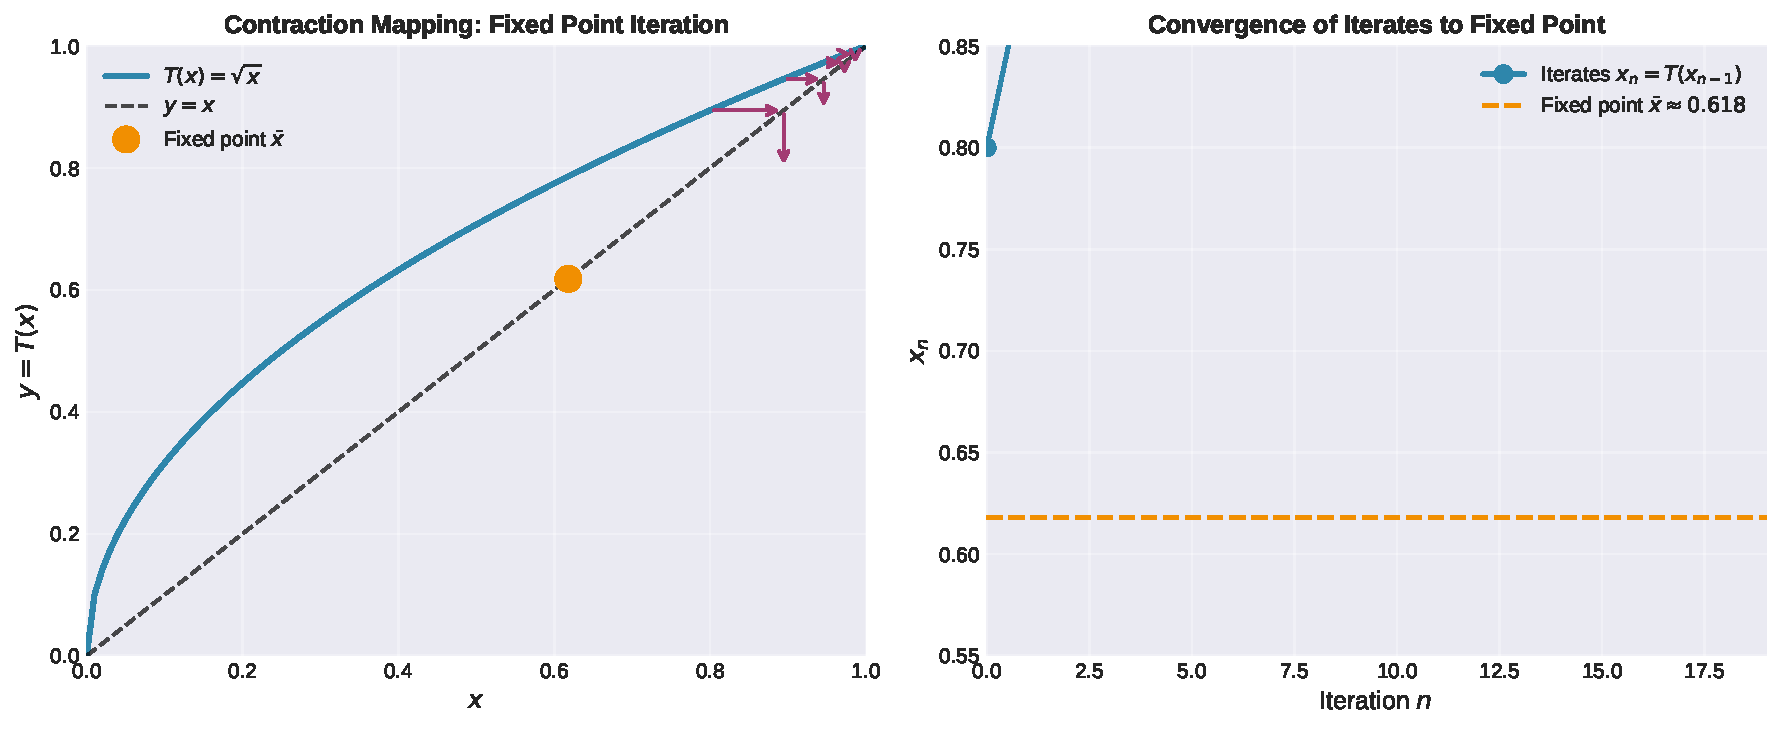
\includegraphics[width=0.65\textwidth]{fig_contraction_fixed_point.pdf}
  \end{center}
\end{frame}

% ==============================================================================
% SECTION 2: OPTIMIZATION IN BANACH SPACES
% ==============================================================================
\section{Optimization in Banach Spaces}

\begin{frame}{Section 7.2: Optimization Problem in Banach Spaces}
  \begin{definition}[Coercive Functional]
    A functional $f: X \to \mathbb{R} \cup \{+\infty\}$ is said to be \textit{coercive} if
    \[
    f(v) \to +\infty \quad \text{as} \quad \|v\|_X \to \infty.
    \]
  \end{definition}

  \vspace{0.5cm}

  \begin{theorem}[Solvability of Unconstrained Minimization]
    Suppose $f: X \to \mathbb{R} \cup \{+\infty\}$ is weakly semicontinuous, coercive, and $f \neq +\infty$. Then the unconstrained minimization problem
    \[
    f(u) = \inf_{v \in X} f(v)
    \]
    admits a solution $u \in X$.
  \end{theorem}

  \vspace{0.3cm}
  \textbf{Sketch of Proof:} Use the compactness of sublevel sets (via coercivity) and weak lower semicontinuity.
\end{frame}

% ==============================================================================
\begin{frame}[allowframebreaks]{Convex Optimization Problems}
  \begin{definition}[Convex Function]
    A function $\varphi: X \to \mathbb{R} \cup \{+\infty\}$ is said to be \textit{convex} if
    \[
    \varphi(\lambda x + (1-\lambda)y) \leq \lambda \varphi(x) + (1-\lambda)\varphi(y)
    \]
    for all $x, y \in X$ and $\lambda \in [0, 1]$.
  \end{definition}

  \vspace{0.5cm}

  \begin{center}
    
\includegraphics[width=0.75\textwidth]{fig_convex_nonconvex.pdf}
  \end{center}

  \framebreak

  \textbf{Properties of Convex Functions:}
  \begin{itemize}
    \item Any local minimum is a global minimum
    \item Sublevel sets are convex
    \item A convex function lies above its tangent hyperplane
    \item Subdifferential is monotone
  \end{itemize}

  \vspace{0.5cm}

  \textbf{Importance in Optimization:}
  \begin{itemize}
    \item Convexity ensures unique global minimizers
    \item Convex optimization problems are computationally tractable
    \item First-order conditions are sufficient for optimality
  \end{itemize}
\end{frame}

% ==============================================================================
% SECTION 3: EKELAND VARIATIONAL PRINCIPLE
% ==============================================================================
\section{Ekeland Variational Principle}

\begin{frame}[allowframebreaks]{Section 7.3: Ekeland Variational Principle}
  \begin{theorem}[Ekeland's Variational Principle (EVP)]
    Let $(M, d)$ be a complete metric space and $f: M \to \mathbb{R} \cup \{+\infty\}$ be a lower semicontinuous function that is bounded below. Let $\varepsilon > 0$ and $\lambda > 0$.

    \textbf{For any $x_0 \in M$ with} $f(x_0) \leq \inf_{x \in M} f(x) + \varepsilon$,

    \textbf{there exists $\bar{x} \in M$ such that:}
    \begin{enumerate}
      \item[(a)] $f(\bar{x}) \leq f(x_0)$
      \item[(b)] $d(x_0, \bar{x}) \leq \frac{\varepsilon}{\lambda}$
      \item[(c)] For all $y \neq \bar{x}$, $f(y) > f(\bar{x}) - \frac{\varepsilon}{\lambda} d(y, \bar{x})$
    \end{enumerate}
  \end{theorem}

  \framebreak

  \begin{center}
    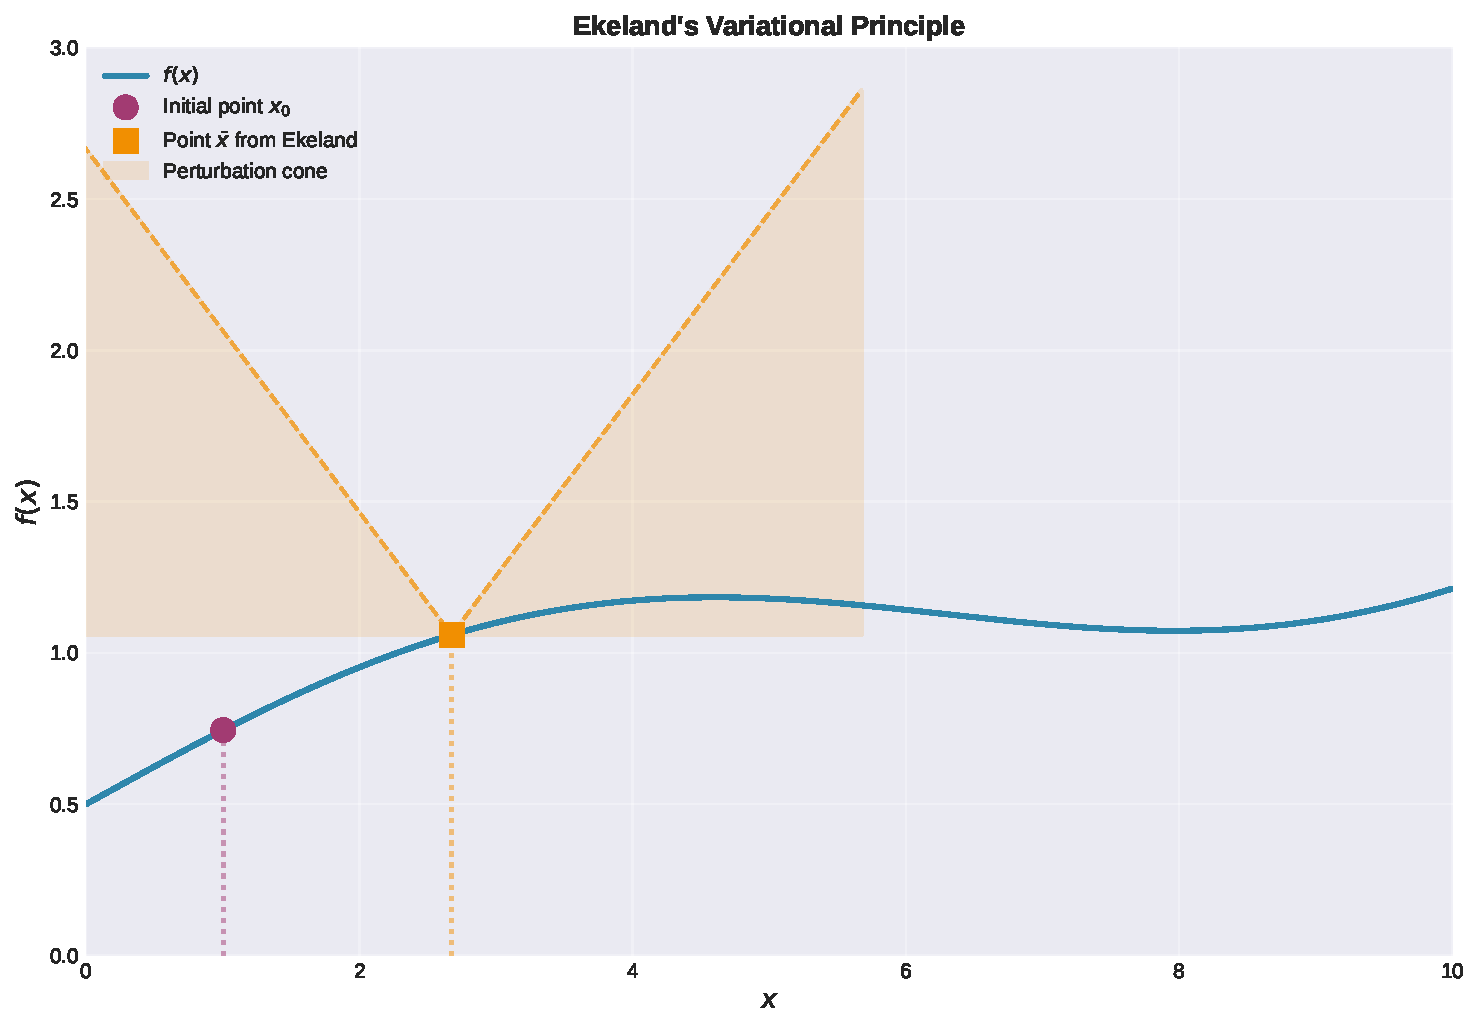
\includegraphics[width=0.8\textwidth]{fig_ekeland_principle.pdf}
  \end{center}

  \vspace{0.3cm}
  \textbf{Geometric Interpretation:} The point $\bar{x}$ is an approximate minimizer of $f$ that perturbs $f$ as little as possible.

  \framebreak

  \textbf{Key Consequences:}
  \begin{itemize}
    \item Ensures existence of approximate minimizers in complete metric spaces
    \item Does not require differentiability or convexity
    \item Applicable to non-smooth optimization problems
    \item Forms the basis for many existence theorems in analysis
  \end{itemize}

  \vspace{0.5cm}

  \textbf{Corollaries:}
  \begin{enumerate}
    \item[(i)] Every lower semicontinuous bounded-below function on a complete metric space has an \textit{infimum} (or comes arbitrarily close to it)
    \item[(ii)] Non-smooth versions exist for Lipschitz functions
    \item[(iii)] Applicable in infinite-dimensional spaces
  \end{enumerate}
\end{frame}

% ==============================================================================
\begin{frame}[allowframebreaks]{Applications of EVP to Fixed Point Theorems}
  \textbf{Connection between Ekeland's Theorem and Fixed Points:}

  Consider the fixed point problem: Find $\bar{x} \in K$ such that $\varphi(\bar{x}) = \bar{x}$.

  Define the function:
  \[
  f(x) = \|\varphi(x) - x\|.
  \]

  If $f$ attains its minimum at some point $\bar{x}$ with $f(\bar{x}) = 0$, then $\bar{x}$ is a fixed point.

  \vspace{0.5cm}

  \textbf{Ekeland's approach:} For any $\varepsilon > 0$, find $\bar{x}_\varepsilon$ such that $f(\bar{x}_\varepsilon) < \varepsilon$ and $\bar{x}_\varepsilon$ is a minimizer of the perturbed function $g_\varepsilon(x) = f(x) + \varepsilon d(x, \bar{x}_\varepsilon)$.

  \framebreak

  \textbf{Theorem [Application to Fixed Points]:}

  Let $K$ be a nonempty closed subset of a Banach space $X$ and $\varphi: K \to K$ a nonexpansive mapping (i.e., $\|\varphi(x) - \varphi(y)\| \leq \|x - y\|$).

  Then for any $x_0 \in K$ and $\varepsilon > 0$, there exists $\bar{x} \in K$ such that
  \begin{enumerate}
    \item $\|\varphi(\bar{x}) - \bar{x}\| < \varepsilon$
    \item $\|\bar{x} - x_0\| < \varepsilon$
  \end{enumerate}

  \vspace{0.3cm}
  \textit{Proof idea:} Apply EVP to $f(x) = \|\varphi(x) - x\|$ and use nonexpansivity to derive the results.

  \framebreak

  \textbf{Remarks:}
  \begin{itemize}
    \item Ekeland's principle provides a unified approach to existence theorems
    \item It shows that minimizers exist as limits of approximate minimizers
    \item The principle works without convexity or smoothness assumptions
    \item Powerful for proving fixed point theorems in infinite-dimensional spaces
  \end{itemize}
\end{frame}

% ==============================================================================
% SECTION 4: VARIATIONAL INEQUALITIES
% ==============================================================================
\section{Variational Inequalities and Fixed Point Problems}

\begin{frame}[allowframebreaks]{Section 7.4: Mappings Associated with Variational Inequality}
  \begin{definition}[Variational Inequality Problem]
    Given a nonempty closed convex set $K \subseteq \mathbb{R}^n$ and a function $f: K \to \mathbb{R}^n$, the \textit{variational inequality problem} (shortly, VI$(K, f)$) is:

    Find $\bar{x} \in K$ such that
    \[
    (x - \bar{x})^T f(\bar{x}) \geq 0 \quad \text{for all } x \in K.
    \]
  \end{definition}

  \vspace{0.5cm}

  \textbf{Intuition:} The vector $f(\bar{x})$ makes an obtuse angle with all feasible directions $(x - \bar{x})$ from $\bar{x}$.

  \framebreak

  \begin{center}
    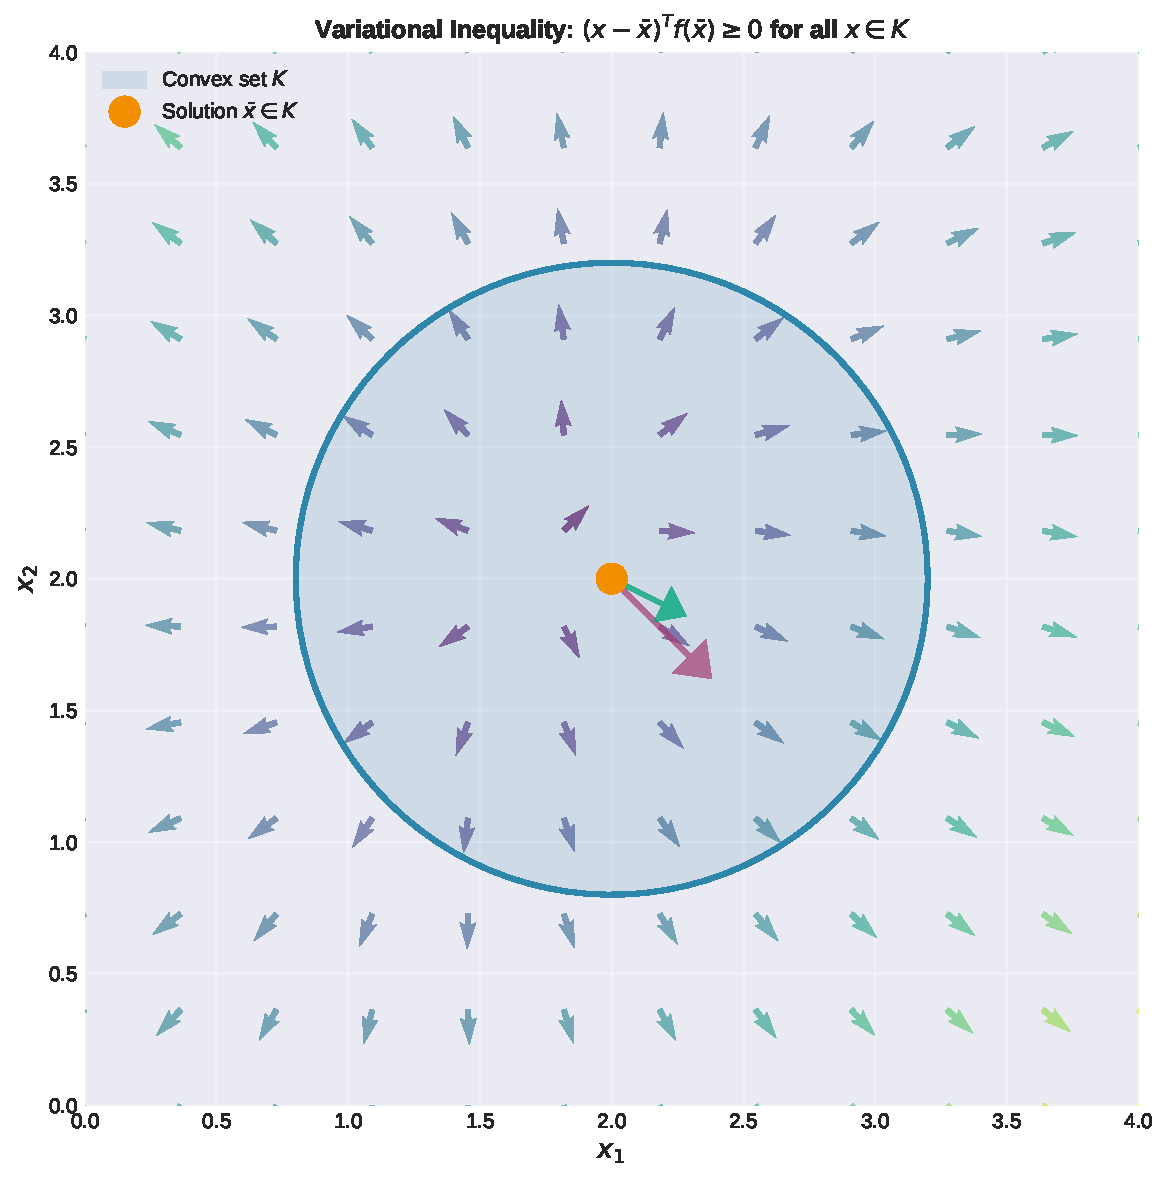
\includegraphics[width=0.75\textwidth]{fig_variational_inequality.pdf}
  \end{center}

  \framebreak

  \textbf{Connection to Optimization:} If $f = \nabla g$ for some differentiable function $g: K \to \mathbb{R}$, then VI$(K, f)$ is equivalent to:
  \[
  g(\bar{x}) \leq g(x) \quad \text{for all } x \in K.
  \]

  \textbf{Connection to Fixed Point Problems:} The variational inequality can be reformulated as a fixed point problem:
  \[
  \bar{x} = P_K(\bar{x} - \alpha f(\bar{x}))
  \]
  where $P_K$ is the projection operator and $\alpha > 0$ is a step size.
\end{frame}

% ==============================================================================
\begin{frame}[allowframebreaks]{Normal Cone and Projection Operator}
  \begin{definition}[Normal Cone]
    Let $K$ be a nonempty closed convex set in $\mathbb{R}^n$. The \textit{normal cone} of $K$ at a point $z \in K$ is
    \[
    N_K(z) = \{v \in \mathbb{R}^n : (y - z)^T v \geq 0 \text{ for all } y \in K\}.
    \]
  \end{definition}

  \vspace{0.5cm}

  \begin{definition}[Projection Operator]
    The \textit{Euclidean projection} of a point $z \in \mathbb{R}^n$ onto the convex set $K$ is
    \[
    P_K(z) = \arg \min_{y \in K} \|z - y\|.
    \]
  \end{definition}

  \framebreak

  \begin{center}
    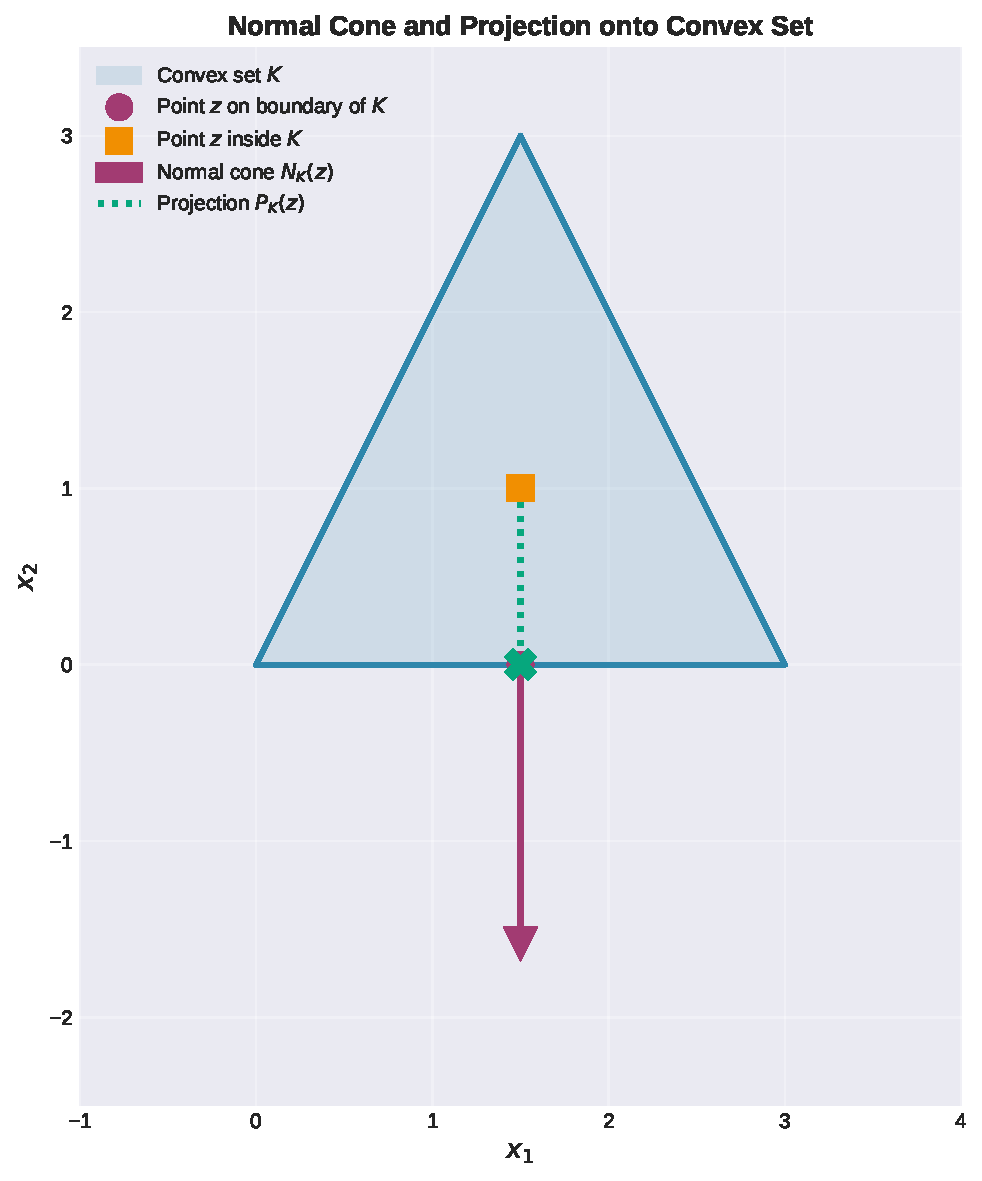
\includegraphics[width=0.75\textwidth]{fig_normal_cone.pdf}
  \end{center}

  \framebreak

  \begin{lemma}
    Let $K$ be a nonempty closed convex set in $\mathbb{R}^n$. For any $z \in \mathbb{R}^n$, the projection $P_K(z)$ exists and is unique. Moreover,
    \[
    (x - P_K(z))^T (P_K(z) - z) \geq 0 \quad \text{for all } x \in K.
    \]
  \end{lemma}

  \vspace{0.3cm}

  \textbf{Significance:} Projection operators are nonexpansive mappings, i.e.,
  \[
  \|P_K(x) - P_K(y)\| \leq \|x - y\| \quad \text{for all } x, y \in \mathbb{R}^n.
  \]
\end{frame}

% ==============================================================================
\begin{frame}[allowframebreaks]{Fixed Point and Variational Inequality Equivalence}
  \textbf{Fundamental Relationship:}

  The variational inequality problem VI$(K, f)$ and the fixed point problem
  \[
  x = P_K(x - \alpha f(x))
  \]
  are \textit{equivalent} for any $\alpha > 0$.

  \vspace{0.5cm}

  \textbf{Proof Sketch:}
  \begin{enumerate}
    \item If $\bar{x}$ solves VI$(K, f)$: $(x - \bar{x})^T f(\bar{x}) \geq 0$ for all $x \in K$
    \item Then: $(\bar{x} - (\bar{x} - \alpha f(\bar{x})))^T \alpha f(\bar{x}) = \alpha \|f(\bar{x})\|^2 \geq 0$
    \item This implies: $\bar{x} - (\bar{x} - \alpha f(\bar{x})) \in N_K(P_K(\bar{x} - \alpha f(\bar{x})))$
    \item Uniqueness of projection yields: $\bar{x} = P_K(\bar{x} - \alpha f(\bar{x}))$
  \end{enumerate}

  \framebreak

  \textbf{Computational Advantage:} This equivalence allows us to:
  \begin{itemize}
    \item Convert variational inequality problems to fixed point problems
    \item Apply fixed point iteration methods to solve variational inequalities
    \item Use projection algorithms for constrained optimization
  \end{itemize}

  \vspace{0.5cm}

  \textbf{Iterative Algorithm (Projected Gradient):}
  \[
  x_{n+1} = P_K(x_n - \alpha f(x_n)) \quad n = 0, 1, 2, \ldots
  \]

  Under suitable conditions (e.g., $f$ is strongly monotone and Lipschitz continuous), this algorithm converges to the unique solution of VI$(K, f)$.
\end{frame}

% ==============================================================================
% NUMERICAL EXAMPLES
% ==============================================================================
\section{Numerical Examples and Applications}

\begin{frame}[fragile]{Example 1: Unconstrained Minimization}
  \textbf{Problem:} Minimize $f(x) = \|Ax - b\|^2_2$ over $\mathbb{R}^n$.

  \vspace{0.3cm}

  \textbf{Gradient:} $\nabla f(x) = 2A^T(Ax - b)$

  \vspace{0.3cm}

  \textbf{Optimality condition:} $A^T(Ax - b) = 0 \Rightarrow A^T A x = A^T b$

  \vspace{0.5cm}

  \begin{lstlisting}[style=mypython]
import numpy as np

# Generate problem data
np.random.seed(42)
m, n = 100, 50
A = np.random.randn(m, n)
b = np.random.randn(m)
x_true = np.random.randn(n)
b = A @ x_true + 0.1 * np.random.randn(m)

# Gradient descent
x = np.zeros(n)
learning_rate = 0.001
for iter in range(100):
    grad = 2 * A.T @ (A @ x - b)
    x = x - learning_rate * grad

# Solution (also can use normal equations)
x_opt = np.linalg.lstsq(A, b, rcond=None)[0]
print(f"GD solution error: {np.linalg.norm(x - x_opt):.6f}")
  \end{lstlisting}
\end{frame}

% ==============================================================================
\begin{frame}{Example 2: Constrained Quadratic Programming}
  \textbf{Problem:} Minimize $\frac{1}{2} x^T Q x + c^T x$ subject to $Ax \leq b$, $x \geq 0$.

  \vspace{0.3cm}

  \textbf{Variational Inequality Formulation:}

  Find $\bar{x} \in K = \{x : Ax \leq b, x \geq 0\}$ such that
  \[
  (y - \bar{x})^T (Q\bar{x} + c) \geq 0 \quad \text{for all } y \in K.
  \]

  \vspace{0.5cm}

  \textbf{Fixed Point Iteration:}
  \[
  x_{n+1} = P_K(x_n - \alpha (Q x_n + c))
  \]
  where $P_K$ is the projection onto the feasible set and $\alpha > 0$ is a step size.

  \vspace{0.5cm}

  \textbf{Convergence:} If $Q$ is positive semidefinite and $\alpha < \frac{2}{\lambda_{\max}(Q)}$, the iteration converges to the unique solution.
\end{frame}

% ==============================================================================
\begin{frame}[fragile]{Example 3: Fixed Point Iteration in Practice}
  \textbf{Problem:} Find a fixed point of $T(x) = 0.6x + 0.5$ (Banach contraction).

  \vspace{0.3cm}

  \begin{lstlisting}[style=mypython]
import numpy as np
import matplotlib.pyplot as plt

# Define the mapping
T = lambda x: 0.6 * x + 0.5

# Fixed point iteration
x = 0.2  # initial point
iterates = [x]
for n in range(30):
    x = T(x)
    iterates.append(x)

# Theoretical fixed point: x* = 0.5/(1-0.6) = 1.25
x_star = 0.5 / (1 - 0.6)

# Plot convergence
plt.figure(figsize=(10, 6))
plt.semilogy(range(len(iterates)),
             np.abs(np.array(iterates) - x_star),
             'o-', label='Error $|x_n - x^*|$')
plt.xlabel('Iteration $n$')
plt.ylabel('Error')
plt.title('Convergence of Fixed Point Iteration')
plt.grid(True, alpha=0.3)
plt.legend()
plt.savefig('convergence.pdf')
  \end{lstlisting}

  \vspace{0.3cm}
  \textbf{Result:} Linear convergence with rate $k = 0.6 < 1$.
\end{frame}

% ==============================================================================
\begin{frame}{Example 4: Projection onto Convex Sets}
  \begin{center}
    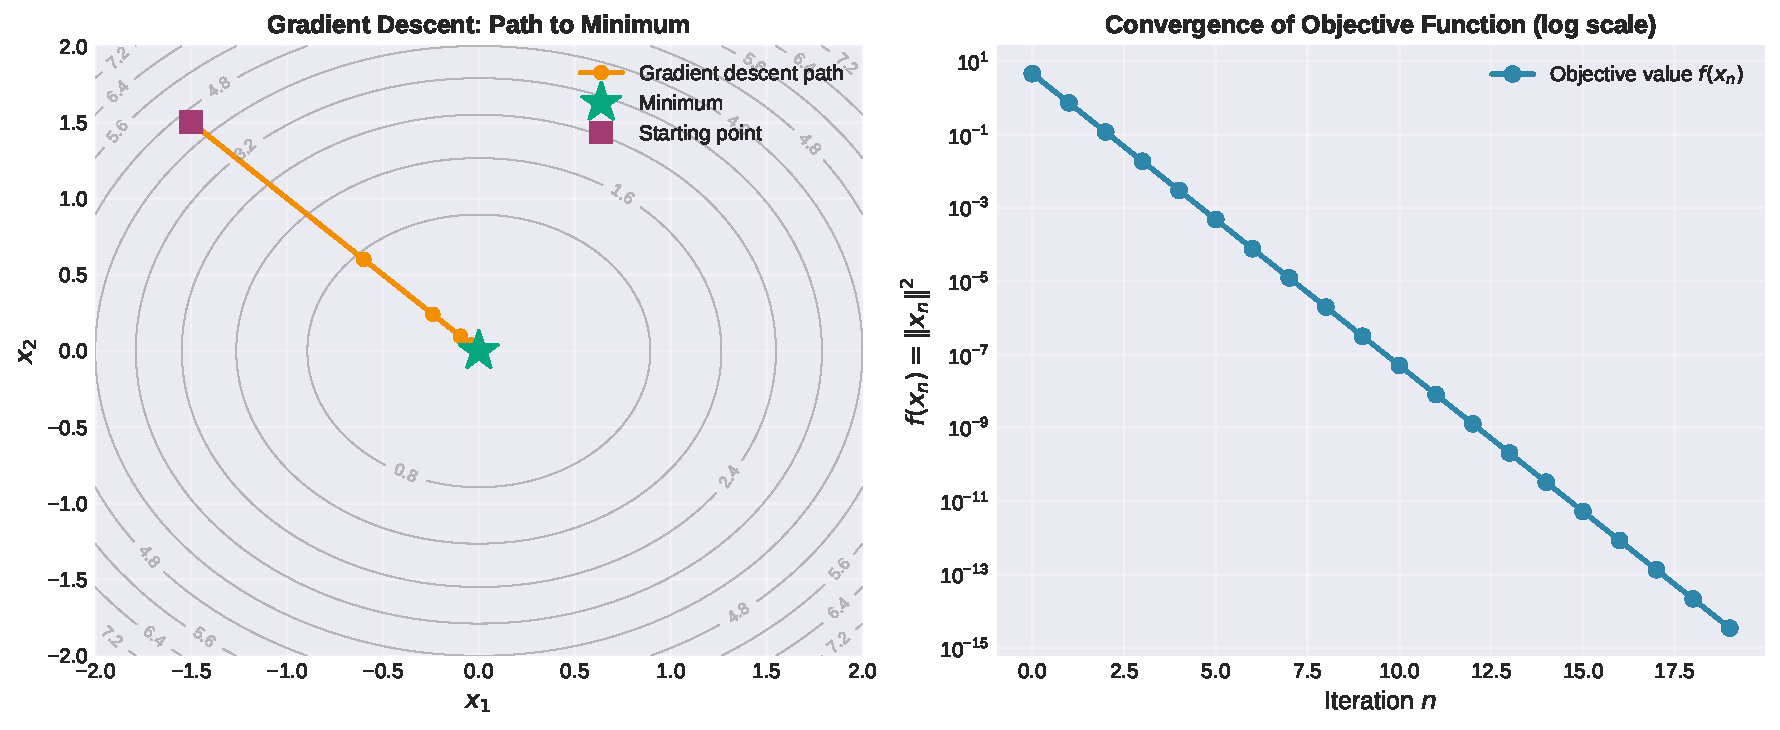
\includegraphics[width=0.75\textwidth]{fig_gradient_descent.pdf}
  \end{center}

  \textbf{Projected Gradient Descent:}
  \[
  x_{n+1} = P_K(x_n - \alpha \nabla f(x_n))
  \]

  Converges under:
  \begin{itemize}
    \item $f$ is convex and differentiable
    \item $\nabla f$ is Lipschitz continuous with constant $L$
    \item Step size satisfies $0 < \alpha < \frac{2}{L}$
  \end{itemize}
\end{frame}

% ==============================================================================
\begin{frame}[allowframebreaks]{Example 5: Banach Contraction Principle Application}
  \begin{center}
    
\includegraphics[width=0.85\textwidth]{fig_banach_contraction.pdf}
  \end{center}

  \framebreak

  \textbf{Key Results from Fixed Point Theory:}

  \begin{theorem}[Banach Fixed Point Theorem]
    Let $(X, d)$ be a complete metric space and $T: X \to X$ be a contraction, i.e.,
    \[
    d(T(x), T(y)) \leq k \, d(x, y) \quad \text{for some } k \in [0, 1) \text{ and all } x, y \in X.
    \]

    Then $T$ has a unique fixed point $\bar{x}^* \in X$, and for any $x_0 \in X$, the sequence $\{x_n\}$ defined by $x_{n+1} = T(x_n)$ converges to $\bar{x}^*$.
  \end{theorem}

  \vspace{0.3cm}

  \textbf{Error Estimate:}
  \[
  d(x_n, \bar{x}^*) \leq \frac{k^n}{1-k} d(x_1, x_0).
  \]

  \textbf{Convergence Rate:} Linear with rate $k$.
\end{frame}

% ==============================================================================
% KEY THEOREMS AND RESULTS
% ==============================================================================
\section{Key Theorems and Results}

\begin{frame}[allowframebreaks]{Summary of Key Theorems}
  \begin{enumerate}
    \item[\textbf{EVP}] \textbf{Ekeland's Variational Principle}: Lower semicontinuous bounded-below functions on complete metric spaces have approximate minimizers.

    \vspace{0.3cm}

    \item[\textbf{BCP}] \textbf{Banach Contraction Principle}: Contractive mappings on complete metric spaces have unique fixed points.

    \vspace{0.3cm}

    \item[\textbf{VI-FP}] \textbf{Variational Inequality-Fixed Point Equivalence}: VI$(K, f)$ is equivalent to the fixed point problem $x = P_K(x - \alpha f(x))$.

    \vspace{0.3cm}

    \item[\textbf{CVX}] \textbf{Convex Optimization}: For convex functions, any local minimum is a global minimum, and first-order conditions are sufficient.
  \end{enumerate}

  \framebreak

  \textbf{Relationships and Connections:}

  \begin{center}
    \begin{tikzpicture}[node distance=2cm, auto]
      \node (ep) [draw, rounded rectangle, minimum width=3cm] {Equilibrium\\Problem};
      \node (mp) [draw, rounded rectangle, minimum width=2cm, below left of=ep] {Minimization};
      \node (spp) [draw, rounded rectangle, minimum width=2cm, below=ep] {Saddle Point};
      \node (nep) [draw, rounded rectangle, minimum width=2cm, below right of=ep] {Nash Eq.};
      \node (fpp) [draw, rounded rectangle, minimum width=2cm, right of=ep] {Fixed Point};
      \node (vi) [draw, rounded rectangle, minimum width=2cm, below right of=fpp] {Var. Ineq.};

      \draw [->] (ep) -- (mp);
      \draw [->] (ep) -- (spp);
      \draw [->] (ep) -- (nep);
      \draw [->] (ep) -- (fpp);
      \draw [->] (fpp) -- (vi);
      \draw [<->] (vi) -- (fpp);
    \end{tikzpicture}
  \end{center}
\end{frame}

% ==============================================================================
\begin{frame}{Existence and Uniqueness Framework}
  \textbf{General Existence Framework:}

  \begin{enumerate}
    \item \textbf{Topological Method}: Use topological degree theory or fixed point theorems
      \begin{itemize}
        \item Brouwer's fixed point theorem
        \item Schauder's fixed point theorem
        \item Leray-Schauder degree
      \end{itemize}

    \vspace{0.3cm}

    \item \textbf{Variational Method}: Use variational principles
      \begin{itemize}
        \item Minimize an associated functional
        \item Apply Ekeland's principle
        \item Use lower semicontinuity and compactness
      \end{itemize}

    \vspace{0.3cm}

    \item \textbf{Monotone Operator Method}: Use properties of monotone operators
      \begin{itemize}
        \item Maximal monotone operators
        \item Subdifferential calculus
        \item Fixed point of resolvents
      \end{itemize}
  \end{enumerate}

  \vspace{0.3cm}

  \textbf{Uniqueness:} Typically follows from:
  \begin{itemize}
    \item Strong monotonicity (for monotone operators)
    \item Strict convexity (for optimization)
    \item Contraction properties (for Banach spaces)
  \end{itemize}
\end{frame}

% ==============================================================================
% APPLICATIONS
% ==============================================================================
\section{Applications}

\begin{frame}{Applications to Real-World Problems}
  \textbf{Optimization:}
  \begin{itemize}
    \item Machine learning (convex optimization, gradient descent)
    \item Portfolio optimization and financial engineering
    \item Resource allocation and production planning
  \end{itemize}

  \vspace{0.3cm}

  \textbf{Variational Inequalities:}
  \begin{itemize}
    \item Traffic flow and network equilibrium problems
    \item Elasticity and plasticity theory
    \item Unilateral contact problems in mechanics
  \end{itemize}

  \vspace{0.3cm}

  \textbf{Fixed Point Applications:}
  \begin{itemize}
    \item Iterative methods for linear and nonlinear systems
    \item Convergence analysis of algorithms
    \item Existence of solutions to differential equations
  \end{itemize}

  \vspace{0.3cm}

  \textbf{Game Theory:}
  \begin{itemize}
    \item Nash equilibrium existence and computation
    \item Evolutionary game dynamics
    \item Mechanism design
  \end{itemize}
\end{frame}

% ==============================================================================
% CONCLUSION
% ==============================================================================
\section{Conclusion}

\begin{frame}[allowframebreaks]{Summary and Conclusions}
  \textbf{Main Takeaways:}

  \begin{enumerate}
    \item Variational methods provide a unified framework for studying optimization and fixed point problems
    \item Ekeland's variational principle is a fundamental tool ensuring existence of approximate solutions
    \item Variational inequalities connect constrained optimization with fixed point theory
    \item Multiple formulations (minimization, equilibrium, fixed point, variational inequality) are equivalent
  \end{enumerate}

  \vspace{0.5cm}

  \textbf{Key Insights:}
  \begin{itemize}
    \item Problems may be transformed to most convenient form
    \item Fixed point iterations provide practical solution methods
    \item Projection operators enable constrained problem-solving
    \item Monotonicity and convexity ensure uniqueness
  \end{itemize}

  \framebreak

  \textbf{Further Reading:}
  \begin{itemize}
    \item Chapters 8-10: Applications to monotone operators and integral equations
    \item Chapters 4-6: Fixed point theorems and degree theory
    \item Chapters 1-3: Functional analysis foundations
  \end{itemize}

  \vspace{0.5cm}

  {\Large \textbf{Thank you!}}

  \vspace{0.3cm}

  Questions and Discussion
\end{frame}

% ==============================================================================
% REFERENCE FRAME
% ==============================================================================
\begin{frame}[allowframebreaks]{References}
  \begin{thebibliography}{99}

    \bibitem{Pathak2018} Pathak, H.K. (2018). \textit{An Introduction to Nonlinear Analysis and Fixed Point Theory}. Springer Nature Singapore.

    \bibitem{Ekeland1974} Ekeland, I. (1974). On the variational principle. \textit{Journal of Mathematical Analysis and Applications}, 47(2), 324-353.

    \bibitem{Boyd2004} Boyd, S., \& Vandenberghe, L. (2004). \textit{Convex Optimization}. Cambridge University Press.

    \bibitem{Rockafellar1970} Rockafellar, R.T. (1970). \textit{Convex Analysis}. Princeton University Press.

    \bibitem{Kinderlehrer1980} Kinderlehrer, D., \& Stampacchia, G. (1980). \textit{An Introduction to Variational Inequalities and Their Applications}. Academic Press.

  \end{thebibliography}
\end{frame}

\end{document}
